\section{Предмети}
\subsection{Валути}
Абстрактна валута: много евтиn, евтин, среден, скъп, много скъп; няма преобразувания.  \\
Луседом Терея: 100 имперски крони = 10 имперски рояла = 1 имперски соверен             \\
Каланор: 100 кралски крони = 10 кралси рояла = 1 кралски соверен                       \\
Сзал Тлея: 13 тъмни монети = 1 черна монета; 900 черни монети = 1 дълбока монета       \\
Креол: 1900 монети за храна = 1 монета за оръжие; 69 монети за оръжие = 1 монета за дом

\subsection{Надници}
Приходи за година. Стойностите в скобите не са ликвидни.
крепостен селянин
страж
ковач
майстор на лъкове
проститутка
лорд-робовладелец
войник
рицар
гробар

% Business / Population required per instance of business (called Support Value or SV)
\rowcolors{1}{white}{lightgray}
\begin{tabular}{p{3cm} | p{2cm}}
обущар      & 150   \\
кожар       & 250   \\
слугиня     & 250   \\
шивач       & 250   \\
бръснар     & 350   \\
бижутер     & 400   \\
таверна     & 400   \\
хлебар      & 500   \\
зидар       & 500   \\
дърводелец  & 550   \\
тъкач       & 600   \\

\end{tabular}

Chandlers     700
Mercers     700
Coopers     700
Bakers                   800
Watercarriers     850
Scabbardmakers   850
Wine-Sellers     900
Hatmakers     950
Saddlers     1,000
Chicken Butchers  1,000
Pursemakers     1,100
Butchers     1,200
Fishmongers     1,200
Beer-Sellers     1,400
Buckle Makers     1,400
Plasterers     1,400
Spice Merchants   1,400
Blacksmiths     1,500
Painters     1,500
Doctors                   1,700*
Roofers       1,800
Locksmiths     1,900
Bathers                   1,900
Ropemakers     1,900
Inns                   2,000
Tanners                   2,000
Copyists    2,000
Sculptors    2,000
Rugmakers    2,000
Harness-Makers  2,000
Bleachers    2,100
Hay Merchants    2,300
Cutlers                  2,300
Glovemakers   2,400
Woodcarvers   2,400
Woodsellers   2,400
Magic-Shops   2,800
Bookbinders   3,000
Illuminators   3,900
Booksellers   6,300
*These are licensed doctors. Total doctor SV is 350.

Some other figures: There will be one noble household per 200 population, one lawyer ("advocate") per 650, one clergyman per 40 and one priest per 25-30 clergy. Businesses not listed here will most likely have an SV from 5,000 to 25,000! The "Magic Shop" means a shop where wizards can purchase spell ingredients, scroll paper and the like, not a place to buy magic swords off the shelf. 
% The SV list was taken (mostly) from the tax list of Paris in 1292, and checked against other sources for accuracy.
% This list can be found in Life in a Medieval City by Joseph and Francis Geis (Harper and Row, 1981).
% This is a fine book by amateur historians, which includes some fascinating descriptions of medieval city life and layout.
% <quoted>

\subsection{Сгради}
\rowcolors{1}{white}{lightgray}
\begin{tabular}{p{3cm} | p{3cm} | p{3cm} | p{3cm} | p{3cm}}
мн. евтин & евтин                                   & среден                   & скъп                           & мн. скъп  \\
щит       & меч                                     & двуръчен меч             & имение                         & замък     \\
брадва    & халчеста къса ризница                   & боен кон                 & пълна броня пазаене 15 здр. 15 &           \\
куче      & кован нагръдник                         & качествена кираса и пола & качествена пълна броня         &           \\
колиба    & къща в малък град или село              & къща в голям град        & централна къща в столицата                 \\
          & магаре С30                              & боен кон                 &
\end{tabular}


\subsection{Оръжия}
\newcommand{\weapon}[8]
{
\begin{multicols}{2}
  \noindent \textbf{#2} \\
  Необходима сила: #3  \\
  Обсег: #4  \\
  Щети: #5  \\
  Свойства: #6  \\
  Маса: #7  \\
  Стойност: #8  \\
  \includegraphics[height=0.13\textheight]{../images/#1}~
\end{multicols}
}

\weapon{knife}{Нож, кама}{3-9}{близък (0.3м)}{ниски (//-2)}{-}{0.3кг}{много евтин}
\weapon{gladius}{Гладиус}{4-10}{среден (0.8м)}{средни (/-2/-2)}{повратливост}{0.8кг}{евтин}
\weapon{rapier}{Рапира}{5-12}{среден (1.2м)}{средни (+2/-2/0)}{}{1кг}{среден}
\weapon{sword}{Меч}{5-12}{среден (0.9м)}{средни (//-2)}{повратливост}{1.1кг}{евтин}
\weapon{longsword}{Дълъг меч}{5-12}{дълъг (1,3м)}{високи (//-2)}{повратливост}{1.5кг}{среден}
\weapon{zweihander}{Цвайхендер}{8-15}{дълъг (2.1м)}{високи (//-2)}{-}{3кг}{среден}

\weapon{small_falx}{Малък фалкс, сърп}{5-12}{среден (0.9м)}{средни/високи (-2/+1/-2)}{закача щит}{1кг}{евтин}
\weapon{falx}{Фалкс}{5-12}{дълъг (1.5м)}{високи (-2/+1/-2)}{закача щит}{1.5кг}{евтин}

\weapon{hand_axe}{Брадвичка}{5-12}{среден (0.8м)}{средни (-1/+1/-1)}{закача щит}{0.8кг}{много евтин}
\weapon{dane_axe}{Датска брадва}{5-12}{среден (1.2м)}{високи (+2/-2/-2)}{бронебойност}{1.5кг}{евтин}
\weapon{helbard}{Алебарда}{5-12}{дълъг (1.7м)}{високи (//)}{бронебойност, поваляне, закача щит}{2.2кг}{евтин}
\weapon{pike}{Пика}{5-12}{отдалечен (7м)}{високи (/-4/-4)}{-}{5кг}{евтин}
\weapon{glavie}{Глейв, нагината}{5-12}{дълъг (2.5м)}{високи (/-1/-2)}{бонус срещу щитове}{1кг}{евтин}
% \weapon{naginata}{Глейв, нагината}{5-12}{дълъг (2.5м)}{високи (/-1/-2)}{бонус срещу щитове}{1кг}{евтин} % !!!!! beautiful [icture, include it some day

\weapon{throwing_knife}{Нож за хвърляне}{3-9}{Сила/2}{ниски (/-4/-4)}{-}{0.2кг}{много евтин}
\weapon{javelin}{Метателно копие}{5-12}{Сила}{средни (/0/0)}{-}{3кг}{много евтин}

\weapon{longbow}{Дълъг лък}{7, зарежда се 1 ход}{Сила*2}{високи (/0/0)}{-}{3кг}{много евтин}
\weapon{arrow}{Бодкин стрела}{-}{+2}{-2}{бронебойност}{0.033кг}{много евтин}
\weapon{arrow}{Широка стрела}{-}{-}{+2}{}{0.033кг}{много евтин}

\weapon{small_crossbow}{Малък арбалет}{7, зарежда се 2 хода}{Сила*2}{високи (/0/0)}{-}{3кг}{евтин}
\weapon{lever_crossbow}{Арбалет}{7 необходима, 9 реална, зарежда се 6 хода}{Сила*2}{високи (/0/0)}{-}{3кг}{евтин}
\weapon{windlass_crossbow}{Арбалет с макара}{7 необходима, 12 реална, зарежда се 12 хода}{Сила*2}{високи (/0/0)}{-}{3кг}{среден}
\weapon{bolt}{Болт}{-}{+2}{-2}{бронебойност}{0.033кг}{много евтин}


\subsection{Old people}


\begin{tabular}{p{2cm} | p{2cm} | p{2cm} | p{2cm} | p{2cm} | p{2cm} | p{2cm}}
Малък арбалет         & 7, зарежда се 2 хода & (Сила х 2) & високи     & бронебойност I & 3кг   & евтин        \\
Арбалет               & 7, зарежда се 2 хода & (Сила х 2) & високи     & бронебойност I & 3кг   & евтин        \\
Арбалет с макара      & 5 необходима, 12 реална, зарежда се 10 хода & (Сила х 2) & високи & бронебойност II & 4кг & среден\\
Колчан 12 стрели      & -                    & -          & -          & -              & 1кг   & много евтин  \\

Бодкин стрела         & -                    & +3         & -3     & бронебойност       & 1.5кг & много евтин  \\
Широка стрела         & -                    & -          & -      &                    & 1.5кг & много евтин  \\
\begin{center}
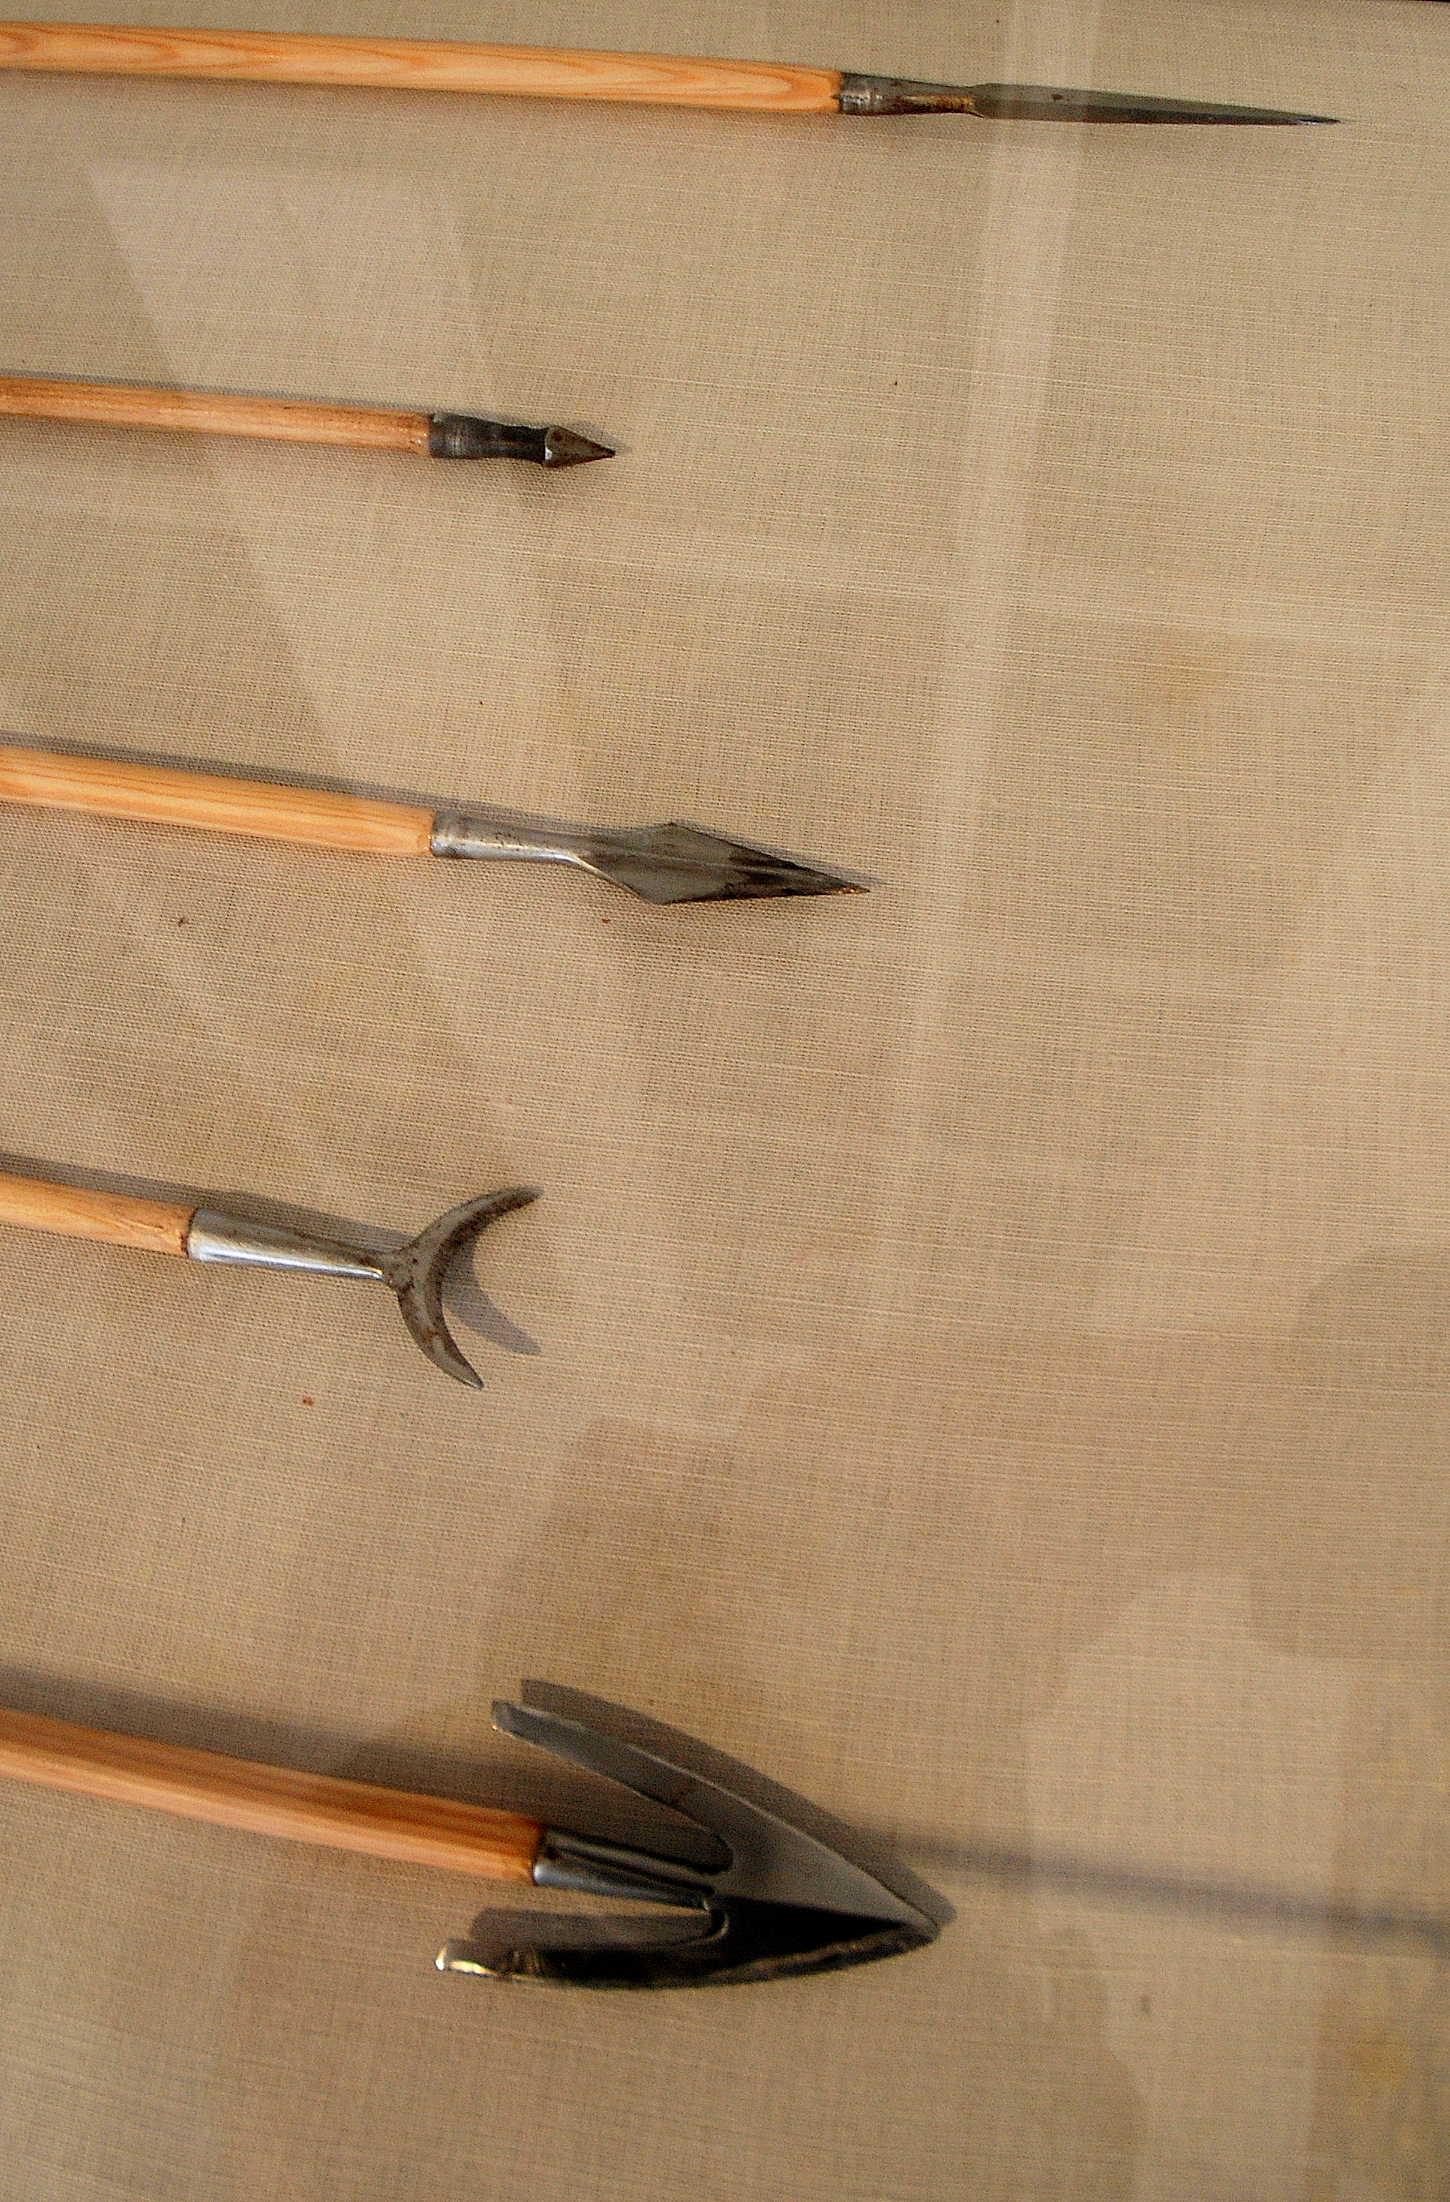
\includegraphics[width=0.75\textwidth]{../images/arrow}~
\\[1cm]
\end{center}

% Щитове.
Дървен щит 80см       & 5-12                 & близък     & ниски      & поваляне       & 2кг   & много евтин  \\
\end{tabular}

\subsection{Брони}
\textbf{Здравина}:
\begin{itemize}[topsep=-0cm, partopsep=0cm, parsep=0cm, itemsep=0cm]
\item{Кожена броня(слоеве памук/хартия/коприна/мека кожа, със зашити плочи варена кожа/хитинова коруба на негъвкавите части) 2}
\item{Халчеста броня, подплатена с гамбезон 4}
\item{Ламенарна броня, подплатена с гамбезон 6}
\item{Лята броня, подплатена с гамбезон(средновековен дизайн - субоптимална форма, субоптимална стомана, примитивно закаляване, подвижност в ставите се осигурява от халчести участъци) 8}
\item{Лята броня, подплатена с гамбезон(ренесансов дизайн - скосени повърхности, качествена стомана (high toughness core),  интелигентно закаляване на повърхностния слой(hardened shell), сложни механични стави) 10}
\\
\\
Масата на конпонент клони към една десета от произведенито на покритието и здравината му за средно качество изработка.
\end{itemize}

\subsection{Други}
комплект отрови - действие за някокко дена \\
алхимични принадлежности - кутия, хаван, стъкленици, лампа и т.н., 2кг, сренед  \\
стрела, клиновидна  \\
стрела, широка  \\
